\documentclass[11pt]{article}
\usepackage[letterpaper,margin=0.78in,top=0.68in,bottom=0.72in]{geometry}
\usepackage{amsmath,amssymb,booktabs,array,tabularx}
\usepackage{xcolor,tikz,microtype,fancyhdr,lastpage}
\usetikzlibrary{arrows.meta,positioning,calc}
\definecolor{navy}{HTML}{17354A}
\definecolor{teal}{HTML}{087E8B}
\definecolor{pale}{HTML}{E7F3F3}
\definecolor{grayfill}{HTML}{EEF1F4}
\definecolor{muted}{HTML}{526778}
\usepackage[unicode,colorlinks=true,urlcolor=teal,linkcolor=teal]{hyperref}
\setlength{\parindent}{0pt}
\setlength{\parskip}{7pt}
\setlength{\emergencystretch}{2em}
\setlength{\headheight}{15pt}
\pagestyle{fancy}\fancyhf{}
\fancyhead[L]{\small\color{muted}OPTIC FLOW \ / \ IMPLEMENTATION GUIDE}
\fancyfoot[L]{\small\color{muted}Visual Attention \& Working Memory}
\fancyfoot[R]{\small\color{muted}\thepage\ / \pageref*{LastPage}}
\renewcommand{\headrulewidth}{0pt}
\newcommand{\heading}[2]{\noindent{\color{teal}\small\bfseries #1}\par\vspace{2pt}{\color{navy}\LARGE\bfseries #2}\par\vspace{5pt}}
\newcommand{\term}[1]{\textbf{\color{navy}#1}}
\begin{document}
\heading{1 / THE WHOLE PIPELINE}{Why the model pads twice}
\textbf{The model adds padding at two different stages because the stages solve two different problems.} First, a border supplies values outside the image when extracting crops near its edges. Later, zeros extend each prepared crop so that FFT correlation handles the tested displacements correctly.

\term{An image} is a rectangular array of pixel values. Here, a grayscale intensity is a number describing brightness: $0$ is black, $1$ is white, and $0.5$ is midpoint gray. The motion pathway receives a $100\times100$ grayscale image at each observation.

\begin{center}
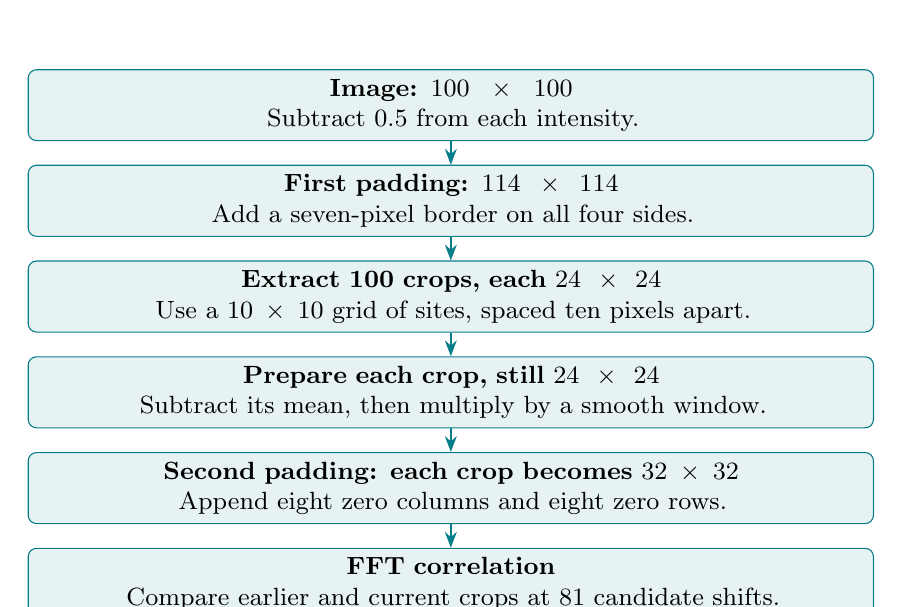
\begin{tikzpicture}[font=\small,box/.style={draw=teal,rounded corners=3pt,fill=pale,text width=10.5cm,align=center,minimum height=0.83cm},arr/.style={-{Stealth[length=2mm]},thick,draw=teal}]
\node[box] (a) {\textbf{Image: $100\times100$}\\Subtract $0.5$ from each intensity.};
\node[box,below=0.30cm of a] (b) {\textbf{First padding: $114\times114$}\\Add a seven-pixel border on all four sides.};
\node[box,below=0.30cm of b] (c) {\textbf{Extract 100 crops, each $24\times24$}\\Use a $10\times10$ grid of sites, spaced ten pixels apart.};
\node[box,below=0.30cm of c] (d) {\textbf{Prepare each crop, still $24\times24$}\\Subtract its mean, then multiply by a smooth window.};
\node[box,below=0.30cm of d] (e) {\textbf{Second padding: each crop becomes $32\times32$}\\Append eight zero columns and eight zero rows.};
\node[box,below=0.30cm of e] (f) {\textbf{FFT correlation}\\Compare earlier and current crops at 81 candidate shifts.};
\foreach \s/\t in {a/b,b/c,c/d,d/e,e/f}{\draw[arr] (\s.south)--(\t.north);}
\end{tikzpicture}
\end{center}
\term{A crop} is a small square of sampled image values. \term{A site} is one fixed position in the grid where the model extracts a crop and computes local motion evidence. The model compares the earlier and current crops from the same site, testing where their image structure best corresponds.

The following pages show exactly where the padding goes, what its values mean, and why the chosen sizes work. Dimensions and operation order follow the repository's \texttt{LocalMotionBank} implementation, checked October 17, 2026.

\newpage
\heading{2 / IMAGE PADDING}{Giving edge crops enough room}
The model divides the $100\times100$ image into ten rows and ten columns of $10\times10$ spatial blocks. Each site uses a larger $24\times24$ crop around its block. The extra extent on each side is
\[
\frac{24-10}{2}=7\text{ pixels}.
\]
Thus, seven pixels of padding on every image edge let the outermost sites obtain complete crops. The padded image has width and height $100+7+7=114$.

\begin{center}
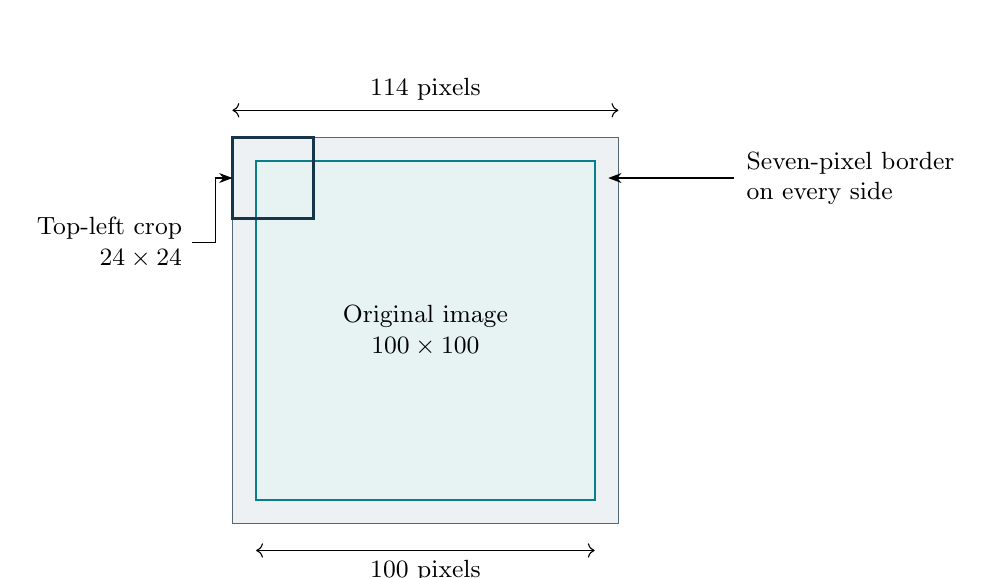
\begin{tikzpicture}[x=0.043cm,y=0.043cm,font=\small]
\filldraw[fill=grayfill,draw=muted] (0,0) rectangle (114,114);
\filldraw[fill=pale,draw=teal,thick] (7,7) rectangle (107,107);
\node[align=center] at (57,57) {Original image\\$100\times100$};
\draw[<->] (0,122)--node[above]{114 pixels}(114,122);
\draw[<->] (7,-8)--node[below]{100 pixels}(107,-8);
\draw[-{Stealth}] (148,102)--(111,102);
\node[anchor=west,align=left] at (149,102) {Seven-pixel border\\on every side};
\draw[draw=navy,very thick] (0,90) rectangle (24,114);
\draw[-{Stealth}] (-12,83)--(-5,83)--(-5,102)--(0,102);
\node[anchor=east,align=right] at (-12,83) {Top-left crop\\$24\times24$};
\end{tikzpicture}
\end{center}

\term{What is the border's brightness?} The code first subtracts $0.5$ from the image, then pads with zeros. In these centered coordinates, zero represents midpoint gray in the original image. For original pixel intensity $I(y,x)$, define the centered value $J(y,x)=I(y,x)-0.5$. Outside the image, the first padding supplies $J=0$.

\term{Where are the crops?} Let $i$ be the grid row and $j$ the grid column, each from $0$ through $9$. Original image coordinates run from $0$ through $99$, with $x$ increasing rightward and $y$ downward. The crop at site $(i,j)$ covers
\[
\boxed{x=10j-7,\ldots,10j+16,\qquad
 y=10i-7,\ldots,10i+16.}
\]
Each inclusive range contains 24 positions. The top-left crop covers coordinates $-7$ through $16$ on each axis; negative coordinates obtain border values. The bottom-right crop covers $83$ through $106$; positions beyond $99$ obtain border values.

\term{Why 100 sites?} A 24-pixel crop moved in steps of ten across a 114-pixel side has $(114-24)/10+1=10$ positions. Ten rows times ten columns give 100 crops. Adjacent horizontal crops share $24-10=14$ columns of pixels. This shared image content is the \emph{overlapping evidence}: nearby sites can observe some of the same structure.

\newpage
\heading{3 / CROP PREPARATION AND FFT PADDING}{Extending the prepared array}
After extraction, the model prepares each crop. Let $P(a,b)$ be one extracted crop, where $a$ is its local row and $b$ its local column, both from $0$ through $23$. Its mean and prepared values are
\[
\mu_P=\frac{1}{576}\sum_{a=0}^{23}\sum_{b=0}^{23}P(a,b),\qquad
A(a,b)=[P(a,b)-\mu_P]h(a)h(b),
\]
\[
h(u)=\tfrac12\left[1-\cos\left(\frac{2\pi u}{23}\right)\right],\quad u=0,\ldots,23.
\]
There are $24\times24=576$ entries in the mean. The function $h$ is a Hann window: it smoothly reduces the weight toward each crop edge, reaching zero at indices $0$ and $23$. Mean subtraction emphasizes brightness variation within the crop; the window emphasizes its interior.

The first padding participates in this preparation. Its initially zero entries are included in the crop mean and are transformed along with the other entries. The second padding is added \emph{after} these operations, so those new entries are exactly zero prepared signal.

\begin{center}
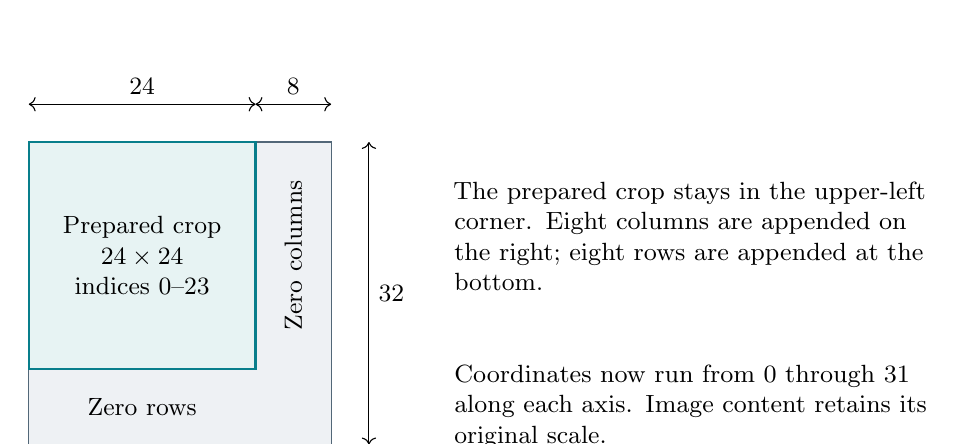
\begin{tikzpicture}[x=0.12cm,y=-0.12cm,font=\small]
\filldraw[fill=grayfill,draw=muted] (0,0) rectangle (32,32);
\filldraw[fill=pale,draw=teal,thick] (0,0) rectangle (24,24);
\node[align=center] at (12,12) {Prepared crop\\$24\times24$\\indices $0$--$23$};
\node[rotate=90] at (28,12) {Zero columns};
\node at (12,28) {Zero rows};
\draw[<->] (0,-4)--node[above]{24}(24,-4);
\draw[<->] (24,-4)--node[above]{8}(32,-4);
\draw[<->] (36,0)--node[right]{32}(36,32);
\node[anchor=west,align=left,text width=6cm] at (44,10) {The prepared crop stays in the upper-left corner. Eight columns are appended on the right; eight rows are appended at the bottom.};
\node[anchor=west,align=left,text width=6cm] at (44,28) {Coordinates now run from $0$ through $31$ along each axis. Image content retains its original scale.};
\end{tikzpicture}
\end{center}

Call the earlier prepared crop $A$ and the current prepared crop $B$. For either crop, the $32\times32$ extension is defined by
\[
\widetilde A(a,b)=
\begin{cases}
A(a,b),&0\leq a<24\text{ and }0\leq b<24,\\
0,&\text{otherwise within the }32\times32\text{ array}.
\end{cases}
\]
The code requests this extension through \texttt{rfft2(patches, s=(32,32))}. Both $A$ and $B$ receive the same placement, so their relative displacement is preserved. This second padding is asymmetric in storage: right and bottom only.

\newpage
\heading{4 / WHY FFT PADDING HELPS}{Preventing an edge from matching the opposite edge}
\term{Correlation} measures agreement between two arrays as one is shifted relative to the other. A candidate displacement is $d=(d_x,d_y)$: $d_x$ is the horizontal shift and $d_y$ is the vertical shift. Positive values mean rightward and downward, respectively.

The model tests each component from $-4$ through $+4$. That is nine horizontal choices and nine vertical choices, giving $9\times9=81$ candidate displacements. Four pixels is the implementation's chosen search radius. The correlation score before energy normalization is
\[
S(d_x,d_y)=\sum_{a=0}^{23}\sum_{b=0}^{23}
A(a,b)\,B_0(a+d_y,b+d_x),
\]
where $B_0$ equals $B$ inside its $24\times24$ crop and equals zero outside it. Each product compares an earlier value with the proposed corresponding current value; the sum aggregates their agreement.

\term{The FFT calculates a circular correlation.} It treats each array axis as periodic: going beyond the last index returns to the first. With an array length $N$, index $-1$ becomes $N-1$. More generally, ``modulo $N$'' means wrapping an index into $0,\ldots,N-1$. For the padded arrays, FFT correlation gives
\[
S_{\mathrm{FFT}}(d_x,d_y)=\sum_{a=0}^{31}\sum_{b=0}^{31}
\widetilde A(a,b)\,
\widetilde B\big((a+d_y)\bmod32,(b+d_x)\bmod32\big).
\]
Padding makes the wrapped positions land in zeros for every shift that the model actually reads.

\term{A one-dimensional example.} Consider two toy rows of length 24. In the earlier row, $A[1]=1$; in the current row, $B[22]=1$. All other entries are zero. Test a displacement of $-3$:

\begin{center}
\renewcommand{\arraystretch}{1.35}
\begin{tabularx}{\linewidth}{@{}>{\raggedright\arraybackslash}p{3.6cm}Xc@{}}
\toprule
Calculation & Position compared with $A[1]$ & Product\\
\midrule
Desired zero extension & $1-3=-2$, outside the crop & $1\cdot0=0$\\
Circular, length 24 & $-2\bmod24=22$, where $B[22]=1$ & $1\cdot1=1$\\
Circular, length 32 & $-2\bmod32=30$, a padded zero & $1\cdot0=0$\\
\bottomrule
\end{tabularx}
\end{center}
Without the extra zeros, the far end of the row creates an apparent match for a small negative shift. The padded computation returns the intended zero score. The same principle applies independently to rows and columns in the two-dimensional crops.

\newpage
\heading{5 / THE NUMBERS AND THE CODE}{Why 32 is enough for the shifts we use}
Only indices $0$ through $23$ can contain nonzero prepared crop values. Adding a tested shift from $-4$ through $+4$ produces indices between $-4$ and $27$. For a length-32 FFT, each possibility has a straightforward interpretation:
\begin{itemize}
\item Indices $0$ through $23$ access the intended crop values.
\item Indices $24$ through $27$ access appended zeros directly.
\item Indices $-4$ through $-1$ wrap to $28$ through $31$, also appended zeros.
\end{itemize}
Thus $S_{\mathrm{FFT}}=S$ for every retained displacement. Applying this argument to both axes establishes the result for all 81 candidate shifts.

For a crop side length $L$ and a tested radius $R$, an FFT side length $N\geq L+R$ supplies enough zero space for this argument. Here $L=24$ and $R=4$, so $28$ would suffice for the retained range. The implementation uses $32$, a power-of-two transform size, which provides eight extra positions per axis. This explains its mathematical adequacy; the code fixes the value directly.

\term{The corresponding operations.} The following condensed code preserves the key ordering. Here \texttt{gray} has already been arranged as a batch of single-channel images.
\begin{quote}\small\ttfamily
centered = gray - 0.5\\
bordered = F.pad(centered, (7, 7, 7, 7))\\
crops = F.unfold(bordered, 24, stride=10)\\
\normalfont\itshape Reshape each extracted crop to 24 by 24.\normalfont\ttfamily\\
prepared = (crops - crop\_means) * hann\_window\\
spectra = torch.fft.rfft2(prepared, s=(32, 32))
\end{quote}
Earlier and current spectra are combined by multiplying the complex conjugate of the earlier spectrum with the current spectrum, then applying the inverse FFT. The implementation selects the 81 requested shifts and normalizes their scores using crop energies. The padding argument above applies to the correlation before that normalization.

\term{Two stages, two meanings for zero.} The image border supplies midpoint-gray values before crop preparation. The FFT extension supplies zero prepared signal after crop preparation. Together they let every spatial site produce comparable local motion evidence, including sites near the image boundaries.

\vspace{3pt}
{\small\textbf{Implementation and API references}\par
[1] \href{https://github.com/jomorg1724/VisualAttentionWorkingMemory/blob/a65838909ee2e7ac169b1f37fc982a2f493c36ed/SecondPass/StabilizedAttentionKrauzlis/model.py#L13-L36}{VisualAttentionWorkingMemory: \texttt{LocalMotionBank}, lines 13--36}. Local implementation checked October 17, 2026.\par
[2] PyTorch, \href{https://docs.pytorch.org/docs/2.14/generated/torch.nn.functional.pad.html}{\texttt{torch.nn.functional.pad}}: padding order and constant padding.\par
[3] PyTorch, \href{https://docs.pytorch.org/docs/2.14/generated/torch.fft.rfft2.html}{\texttt{torch.fft.rfft2}}: transform size \texttt{s} pads or trims the input to the requested dimensions.}
\end{document}
